\documentclass[12pt,a4paper]{article}

%\usepackage[left=1.5cm,right=1.5cm,top=1cm,bottom=2cm]{geometry}
\usepackage[in, plain]{fullpage}
\usepackage{array}
%\usepackage{../../pas-math}
\usepackage{../../moncours}



%-------------------------------------------------------------------------------
%          -Packages nécessaires pour écrire en Français et en UTF8-
%-------------------------------------------------------------------------------
\usepackage[utf8]{inputenc}
\usepackage[frenchb]{babel}
%\usepackage{numprint}
\usepackage[T1]{fontenc}
%\usepackage{lmodern}
\usepackage{textcomp}
\usepackage[french, boxed]{algorithm2e}
\usepackage{hyperref}


%-------------------------------------------------------------------------------

%-------------------------------------------------------------------------------
%                          -Outils de mise en forme-
%-------------------------------------------------------------------------------
\usepackage{hyperref}
\hypersetup{pdfstartview=XYZ}
%\usepackage{enumerate}
\usepackage{graphicx}
\usepackage{multicol}
\usepackage{tabularx}
\usepackage{multirow}
\usepackage{color}
\usepackage{eurosym}


\usepackage{anysize} %%pour pouvoir mettre les marges qu'on veut
%\marginsize{2.5cm}{2.5cm}{2.5cm}{2.5cm}

\usepackage{indentfirst} %%pour que les premier paragraphes soient aussi indentés
\usepackage{verbatim}
\usepackage{enumitem}
\usepackage{booktabs}
\usepackage[usenames,dvipsnames,svgnames,table]{xcolor}

\usepackage{variations}

%-------------------------------------------------------------------------------


%-------------------------------------------------------------------------------
%                  -Nécessaires pour écrire des mathématiques-
%-------------------------------------------------------------------------------
\usepackage{amsfonts}
\usepackage{amssymb}
\usepackage{amsmath}
\usepackage{amsthm}
\usepackage{tikz}
\usepackage{xlop}
\usepackage[output-decimal-marker={,}]{siunitx}
%-------------------------------------------------------------------------------

%-------------------------------------------------------------------------------
%                  -Nécessaires pour écrire des formules chimiquess-
%-------------------------------------------------------------------------------

\usepackage[version=4]{mhchem}

%-------------------------------------------------------------------------------
% Pour pouvoir exploiter les fichiers directement dans beamer
\newcommand{\pause}{\ }
%-------------------------------------------------------------------------------
%                    - Mise en forme avancée
%-------------------------------------------------------------------------------

\usepackage{ifthen}
\usepackage{ifmtarg}


\newcommand{\ifTrue}[2]{\ifthenelse{\equal{#1}{true}}{#2}{$\qquad \qquad$}}

%\newcommand{\kword}[1]{\textcolor{red}{\underline{#1}}}
%-------------------------------------------------------------------------------

%-------------------------------------------------------------------------------
%                     -Mise en forme d'exercices-
%-------------------------------------------------------------------------------
%\newtheoremstyle{exostyle}
%{\topsep}% espace avant
%{\topsep}% espace apres
%{}% Police utilisee par le style de thm
%{}% Indentation (vide = aucune, \parindent = indentation paragraphe)
%{\bfseries}% Police du titre de thm
%{.}% Signe de ponctuation apres le titre du thm
%{ }% Espace apres le titre du thm (\newline = linebreak)
%{\thmname{#1}\thmnumber{ #2}\thmnote{. \normalfont{\textit{#3}}}}% composants du titre du thm : \thmname = nom du thm, \thmnumber = numéro du thm, \thmnote = sous-titre du thm

%\theoremstyle{exostyle}
%\newtheorem{exercice}{Exercice}
%
%\newenvironment{questions}{
%\begin{enumerate}[\hspace{12pt}\bfseries\itshape a.]}{\end{enumerate}
%} %mettre un 1 à la place du a si on veut des numéros au lieu de lettres pour les questions 
%-------------------------------------------------------------------------------

%-------------------------------------------------------------------------------
%                    - Mise en forme de tableaux -
%-------------------------------------------------------------------------------

\renewcommand{\arraystretch}{1.7}

\setlength{\tabcolsep}{1.2cm}

%-------------------------------------------------------------------------------



%-------------------------------------------------------------------------------
%                    - Racourcis d'écriture -
%-------------------------------------------------------------------------------
%Droites
\newcommand{\dte}[1]{$(#1)$}
\newcommand{\fig}[1]{figure $#1$}
\newcommand{\sym}{symétrique}
\newcommand{\syms}{symétriques}
\newcommand{\asym}{axe de symétrie}
\newcommand{\asyms}{axes de symétrie}
\newcommand{\seg}[1]{$[#1]$}
\newcommand{\monAngle}[1]{$\widehat{#1}$}
\newcommand{\bissec}{bissectrice}
\newcommand{\mediat}{médiatrice}
\newcommand{\ddte}[1]{$[#1)$}


% Angles orientés (couples de vecteurs)
\newcommand{\aopp}[2]{(\vec{#1}, \vec{#2})} %Les deuc vecteurs sont positifs
\newcommand{\aopn}[2]{(\vec{#1}, -\vec{#2})} %Le second vecteur est négatif
\newcommand{\aonp}[2]{(-\vec{#1}, \vec{#2})} %Le premier vecteur est négatif
\newcommand{\aonn}[2]{(-\vec{#1}, -\vec{#2})} %Les deux vecteurs sont négatifs

%Ensembles mathématiques
\newcommand{\naturels}{\mathbb{N}} %Nombres naturels
\newcommand{\relatifs}{\mathbb{Z}} %Nombres relatifs
\newcommand{\rationnels}{\mathbb{Q}} %Nombres rationnels
\newcommand{\reels}{\mathbb{R}} %Nombres réels
\newcommand{\complexes}{\mathbb{C}} %Nombres complexes


%Intégration des parenthèses aux cosinus
\newcommand{\cosP}[1]{\cos\left(#1\right)}
\newcommand{\sinP}[1]{\sin\left(#1\right)}


%Probas stats
\newcommand{\stat}{statistique}
\newcommand{\stats}{statistiques}


\newcommand{\homo}{homothétie}
\newcommand{\homos}{homothéties}


\newcommand{\mycoord}[3]{(\textcolor{red}{\num{#1}} ; \textcolor{Green}{\num{#2}} ; \textcolor{blue}{\num{#3}})}
%-------------------------------------------------------------------------------

%-------------------------------------------------------------------------------
%                    - Mise en page -
%-------------------------------------------------------------------------------

\newcommand{\twoCol}[1]{\begin{multicols}{2}#1\end{multicols}}


\setenumerate[1]{font=\bfseries,label=\textit{\alph*})}
\setenumerate[2]{font=\bfseries,label=\arabic*)}


%-------------------------------------------------------------------------------
%                    - Elements cours -
%-------------------------------------------------------------------------------

%Correction d'exercice
\newcommand{\exoSec}[2]{\subsection*{Exercice #1 page #2}}
%-------------------------------------------------------------------------------
%                    - raccourcis d'écriture -
%-------------------------------------------------------------------------------

%Mise en évidence de termes clés
\newcommand{\mykw}[1]{\textcolor{red}{\underline{\textbf{#1}}}}

%Exercices
\newcommand{\exo}[2]{exercice #1 page #2}
\newcommand{\Exo}[2]{Exercice #1 page #2}

\renewcommand{\pause}{\ }

%Intervalles
\newcommand{\interOO}[2]{$]$#1 , #2$[$}
\newcommand{\interOF}[2]{$]$#1 , #2$]$}
\newcommand{\interFO}[2]{$[$#1 , #2$[$}
\newcommand{\interFF}[2]{$[$#1 , #2$]$}





\date{}
\title{}

\graphicspath{{./img/}}


\begin{document}
	
	
\chap[num=5, color=blue]{\small Comment se propage la lumière et se forment les ombres ?}{ }	

\section{Propagation de la lumière}

\begin{myact}{}
	Activité 19 page 59 cahier d'activités : Différentes formes d'énergie et leurs sources.
	 
	Activité 3 page 136 le livret scolaire : Énergies renouvelables. 
\end{myact}

\begin{mybilan}
	\begin{itemize}
		\item Un \kw{solide} a une \kw{forme propre} qui ne change pas, on peut le saisir.
		\item Un \kw{liquide} prend la \kw{forme du récipient} qui le contient.
		\item La surface d'un liquide en contact avec l'air est sa \kw{surface libre}.
		\item Au repos, cette surface libre est \kw{plane et horizontale}.
	\end{itemize}	   
\end{mybilan}



%
%\begin{myexos}
%	\begin{itemize}
%		\item \exo{1}{84}
%		\item \exo{6}{85}
%	\end{itemize}
%\end{myexos}

\section{Modélisation du trajet de la lumière}

\begin{myact}{2 page 153}
	\begin{enumerate}
		\item Sur la fiole jaugée, le volume est exprimé en millilitres ($mL$). \pause
		\item La fiole jaugée contient \num{1000} $mL$ de liquide, soit 1 litre ($L$). \pause
		\item Le volume du récipient cubique est de 1 décimètre cube ($dm^3$). \pause
		\item On nous indique que le contenu de la fiole jaugée a été transféré sans perdre de liquide, donc le volume n'a pas changé.\pause
		\item Le récipient cubique contient 1 $dm^3$ de liquide, soit \num{1000} centimètres cubes ($cm^3$).\pause
		\item On a 1 $L =$ 1 $dm^3$ et 1 $mL = $ 1 $cm^3$.
	\end{enumerate}
\end{myact}

\begin{mybilan}
	Pour décrire la vitesse d'un objet en mouvement, on utilise trois caractéristiques :
	\begin{itemize}
		\item la \kw{direction} (horizontale, verticale ou oblique), tangente à la trajectoire;
		
		\item le \kw{sens}, celui du mouvement (vers la gauche, vars la droite, vers le haut etc.);
		
		\item la \kw{valeur} exprimée m/s (ou km/h ou autre).
		
		Si le mouvement est uniforme, la relation \kw{$ v = \dfrac{d}{\Delta t} $}, permet de relier la vitesse de l'objet, la distance parcourue et la durée du parcours avec :
		\begin{itemize}
			\item d : distance parcourue en mètre (m)
			\item $\Delta t$ :durée du trajet en seconde (s)
			\item v : vitesse en mètre par seconde (m/s).
		\end{itemize}
	\end{itemize}



\end{mybilan}



%\begin{myexos}
%	\begin{multicols}{2}
%	
%		\begin{itemize}
%			\item \exo{2}{84}
%			\item \exo{7}{85}
%			
%		\end{itemize}
%	
%	\end{multicols}
%\end{myexos}


\section{Zone éclairée et zone d'ombre}

\begin{myact}{3 page 64}
	\begin{enumerate}\pause
		\item Dans une salle obscure, on ne voit pas la lumière entre le projecteur et le cône.\pause
		\item On observe une zone éclairée sur le cône.\pause
		\item Lorsque l'on saupoudre de la craie entre le projecteur et le cône on observe des grains de craie éclairés.\pause
		\item Si les grains ne sont pas dans la lumière, ils n'en reçoivent pas et ne sont donc pas visibles.\pause
		\item Dans cette expérience, les grains de craie sont des objets diffusants.\pause
		\item La lumière n'est visible que si on place des objets diffusants sur son trajet.
	\end{enumerate}
\end{myact}

\begin{mybilan}
	
	\twoCol{
	\begin{center}
		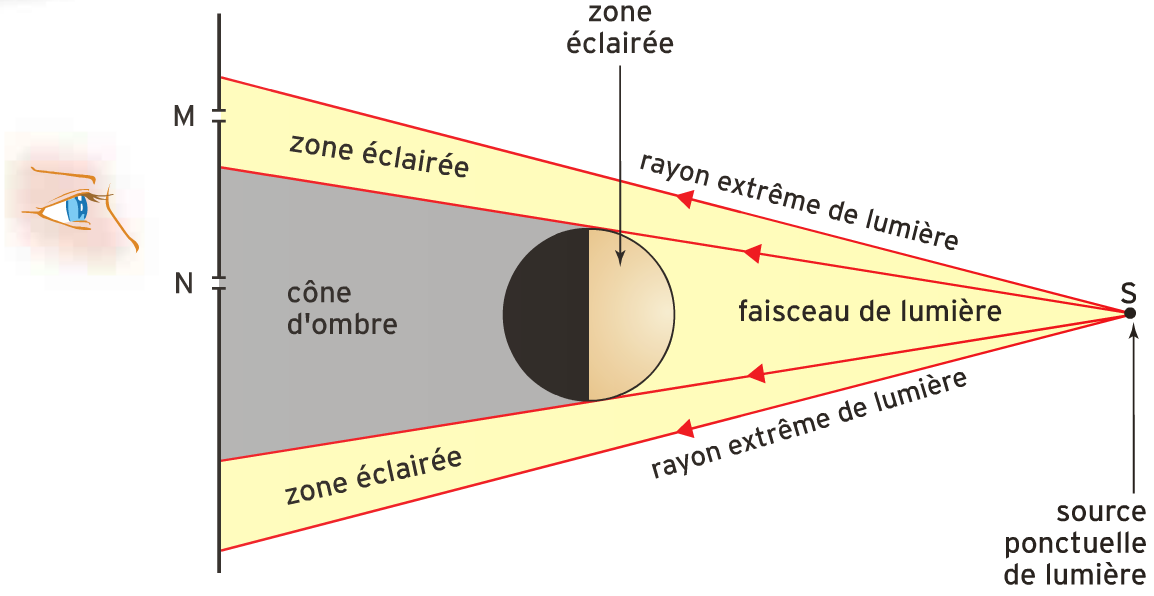
\includegraphics[scale=0.7]{bilan3}
	\end{center}

	\begin{itemize}
		\item Une tension est \kw{périodique} lorsque ses \kw{variations se répètent} identiques à elles mêmes au cours du temps. 
		\item La \kw{durée} d'un motif est la \kw{période}. On la note $T$, son unité est la seconde $s$.
	\end{itemize}
	}

\end{mybilan}

%\begin{myexos}
%	\begin{itemize}
%		\item \exo{3}{84}
%		\item \exo{8}{85}
%	\end{itemize}
%\end{myexos}
%

\section{Ombre propre et ombre portée}



\begin{myact}{4 page 155}
	\begin{enumerate}
		\item L'unité de la température mesurée par la sonde du thermomètre électronique est le degré Celsius (°$C$). \pause
		\item La température du liquide contenu dans le bécher est de \num{17.4} °$C$.\pause
		\item L'intervalle entre deux graduations du thermomètre est alcool correspond à 1 °$C$.\pause
		\item Il faut laisser à la sonde le temps de mesurer précisément la température du liquide, c'est pourquoi on attend que l'affichage se stabilise.\pause
		\item Le réservoir du thermomètre à alcool doit être complètement immergé dans le liquide car c'est lui qui sert à <<mesurer>> la température.\pause
		\item La température mesurée par le thermomètre à alcool est de $17$ °$C$.		
	\end{enumerate}
\end{myact}


\begin{mybilan}
	\begin{itemize}
		\item La masse d'un corps est \kw{proportionnelle} à son volume; \pause
		\item Le coefficient de proportionnalité est la \kw{masse volumique} (notée $\rho$);\pause
		\item \kw{Un litre d'eau} a une masse de \kw{1 kilogramme};\pause
		\item Une substance est \kw{plus dense} qu'une autre si, pour un même volume, sa masse est supérieure.		
	\end{itemize}
\end{mybilan}

%\begin{myexos}
%	\twoCol{\begin{itemize}
%		\item \exo{4}{84}
%		\item \exo{10}{86}
%		\item \exo{11}{86}
%		\item \exo{13}{86}
%	\end{itemize}}
%\end{myexos}

\end{document}]